\begin{figure}[p]
\centering\begin{singlespace}
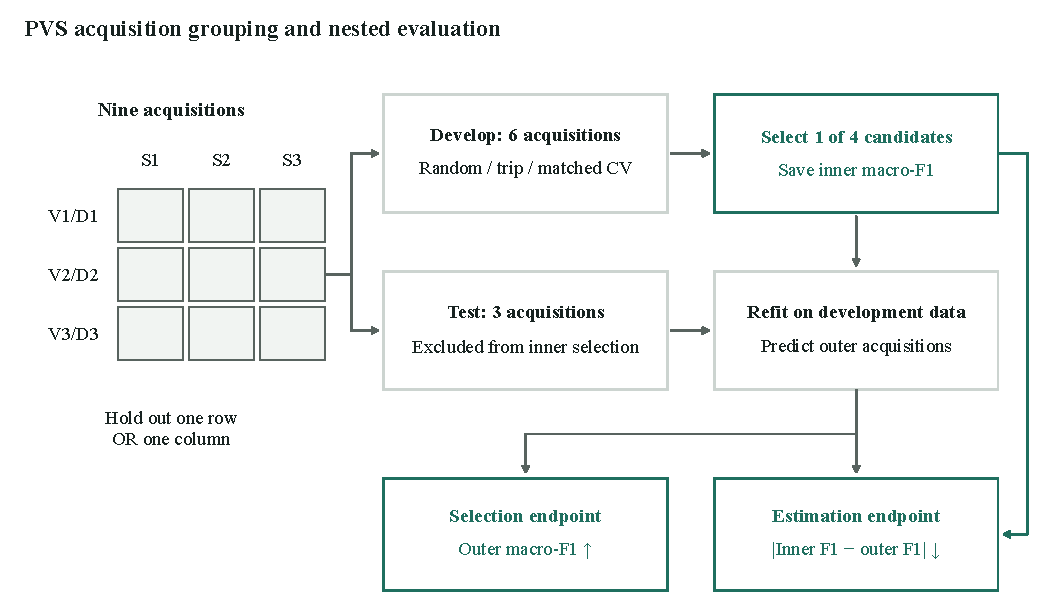
\includegraphics[width=\linewidth]{figures/pvs_evaluation_workflow_v14.pdf}
\caption{PVS acquisition grouping and nested evaluation. Each cell is one acquisition; S denotes scenario and V/D a vehicle/driver pair. A vehicle/driver-held-out fold excludes a row and a scenario-held-out fold a column. Each selector chooses among four candidates by pooled inner OOF macro-F1 on six development acquisitions. The saved estimate and the same candidate's outer score define an absolute error, averaged across three domains per axis. Refitting uses development data only. Vehicle and driver effects are linked, and both axes reuse nine acquisitions.}
\label{fig:pvs-workflow}
\end{singlespace}\end{figure}
\clearpage
\begin{figure}[p]
\centering\begin{singlespace}
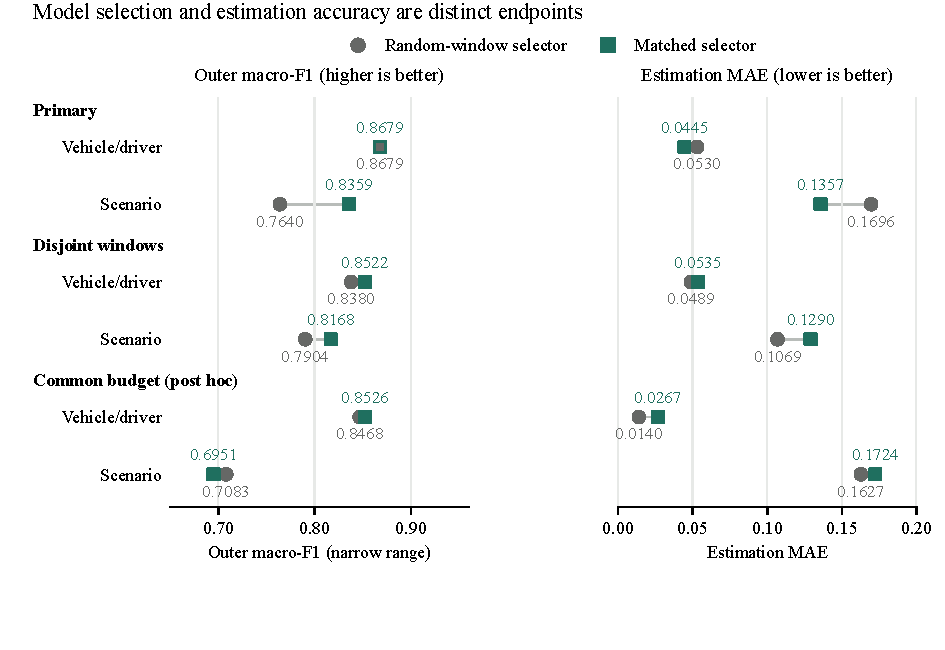
\includegraphics[width=\linewidth]{figures/pvs_endpoints_ijpe.pdf}
\caption{PVS selected-model classification performance and estimation error. Grey circles denote random-window selection and teal squares matched-domain selection. Segments connect selector summaries within the same analysis and held-out axis. Values are three-domain means from the same nine acquisitions. Primary and disjoint-window rows use full-development outer refits; the post hoc common-budget rows use equally budgeted outer refits. The left axis is restricted to 0.65--0.96 and the right starts at zero. The declared MAE-reduction requirement of at least 0.02 on both axes is unmet.}
\label{fig:pvs-endpoints}
\end{singlespace}\end{figure}
\clearpage
\begin{figure}[p]
\centering\begin{singlespace}
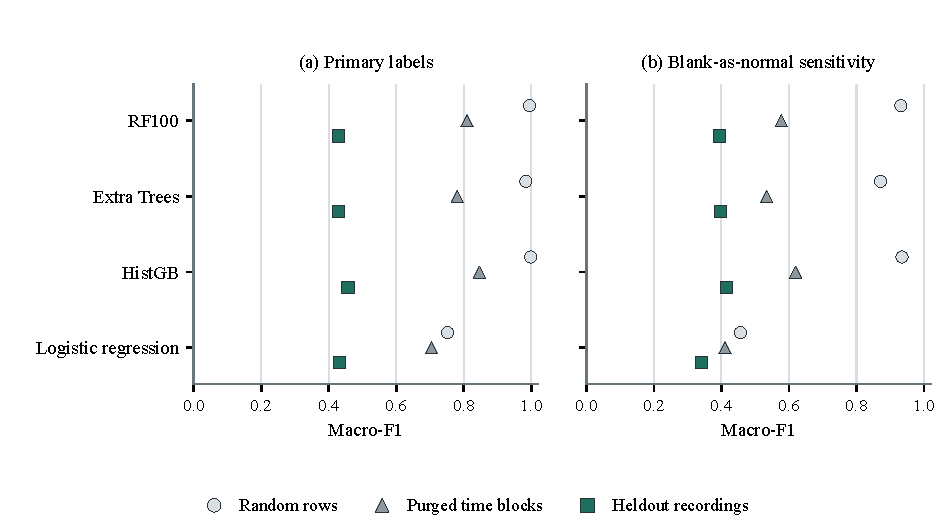
\includegraphics[width=\linewidth]{figures/main_a_ijpe.pdf}
\caption{RoadSens full-numeric five-fold mean macro-F1 across four classifiers and three evaluation scales. Symbols denote point estimates; the same sources contribute to the three split designs. Exact values are in Table~\ref{tab:main}.}
\label{fig:roadsens}
\end{singlespace}\end{figure}
